% 乙醇实际测量结果，接在查看器点选与读数步骤之后。
\begin{figure}[H]
\centering
\begin{minipage}[t]{62mm}
\vspace{0pt}
% 测量卡片(55,328,845,1717)，790×1389；62mm约324ppi。
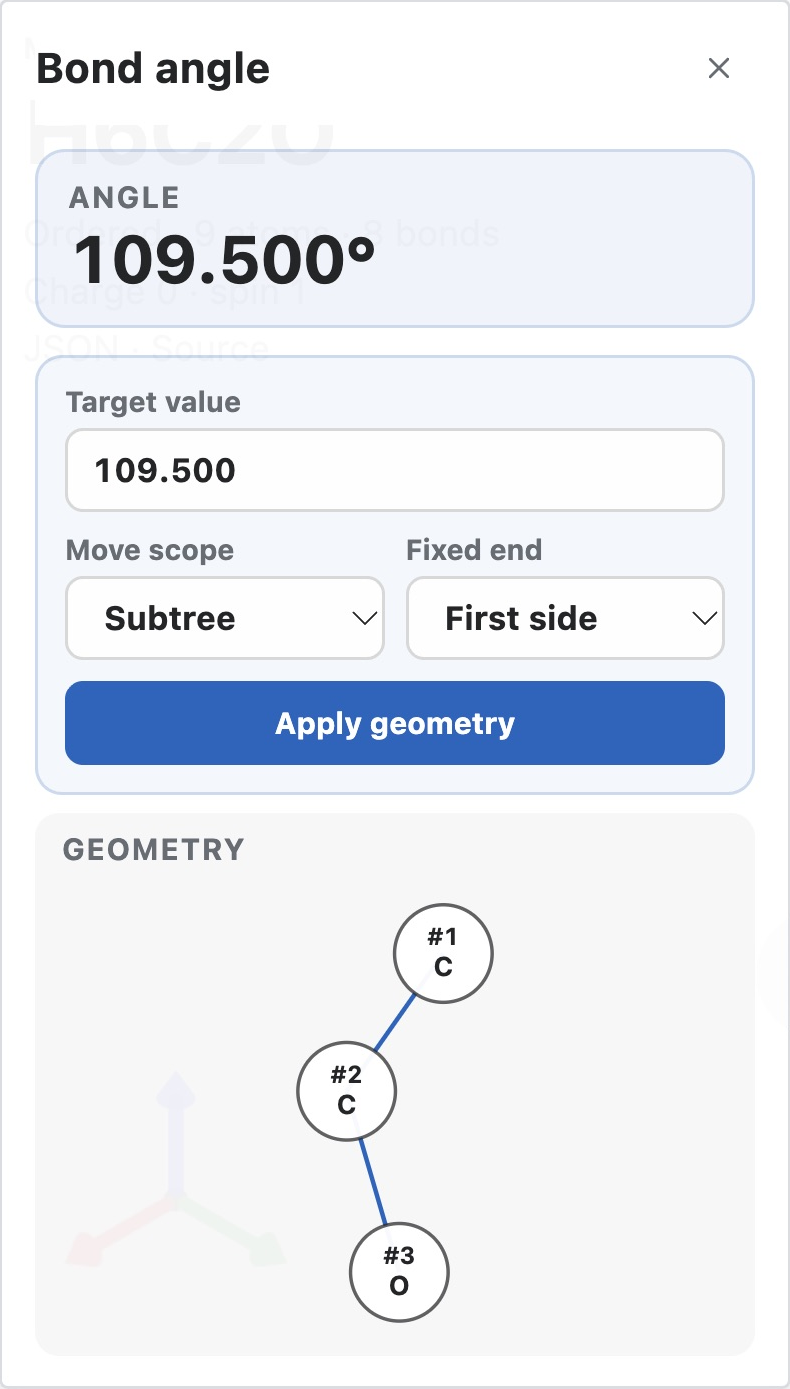
\includegraphics[width=\linewidth]{publication-assets/crop-cdb0f92bdcdbb307f144.png}
\end{minipage}\hfill
\begin{minipage}[t]{58mm}
\vspace{0pt}
% 三重原子和实际角线(850,400,2000,1650)，1150×1250；58mm约504ppi。
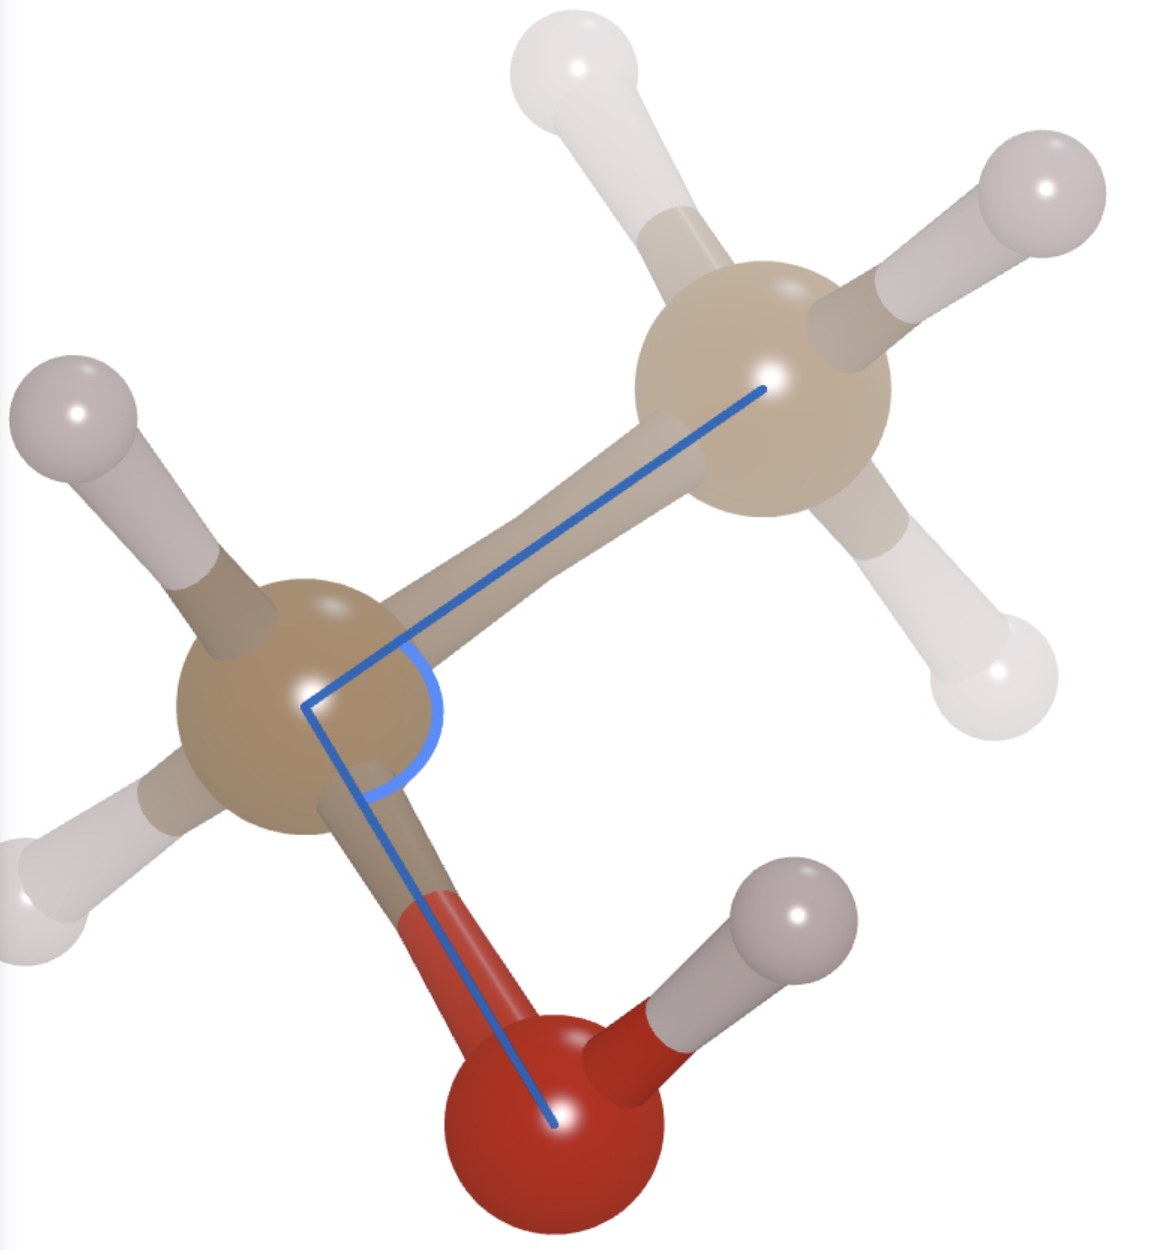
\includegraphics[width=\linewidth]{publication-assets/crop-4185f48c89b2b877f7b1.png}
\end{minipage}
\caption{应用后使用查看器\ui{Bond angle}进行的实际测量。左侧读数为$109.500^\circ$，路径为\#1 C、\#2 C、\#3 O；右侧保留三个重原子和相应角线。本次从\file{ethanol-optimized.json}另载副本，再将该角设为$109.5^\circ$，并非把这一练习值作为优化平衡角。}
\label{fig:ethanol-angle-measured}
\end{figure}
